% Author: Nikita Moiseev <xmoise01@stud.fit.vutbr.cz>
% Author: Elena Marochkina <xmaroc00@stud.fit.vutbr.cz>
% Author: Nikita Pasynkov <xpasyn0034@stud.fit.vutbr.cz>


\documentclass[a4paper, 11pt]{article}

\usepackage[czech]{babel}
\usepackage[utf8]{inputenc}
\usepackage{geometry}
\usepackage{placeins}
\geometry{verbose,a4paper,tmargin=2cm,bmargin=2cm,lmargin=2.5cm,rmargin=1.5cm}
\usepackage{times}
\renewcommand{\baselinestretch}{1.5}
\usepackage{geometry}
\usepackage{verbatim}
\usepackage{enumitem}
\usepackage{graphicx} % insert picture
\usepackage[unicode]{hyperref}
\usepackage[table,xcdraw]{xcolor}
\usepackage{indentfirst}
\usepackage[T1]{fontenc}
\setlength{\parskip}{0.5cm}
\def\code#1{\texttt{#1}}
\setcounter{secnumdepth}{4}
\usepackage[raggedright]{titlesec}
\titleformat{\paragraph}[hang]{\normalfont\normalsize\bfseries}{\theparagraph}{1em}{}
\titlespacing*{\paragraph}{0pt}{3.25ex plus 1ex minus .2ex}{0.5em}
% \newcommand{\myparagraph}[1]{\paragraph{#1}\mbox{}}
\documentclass[xcolor=table]{beamer}
\hypersetup{
	colorlinks = false,
	hypertexnames = false,
	citecolor = blue
}
\usepackage{pdflscape}

\begin{document}
	%% Title page %%
	\begin{titlepage}
		\begin{center}
			\includegraphics[width=0.77\linewidth]{fit_logo.png} \\

			\vspace{\stretch{0.382}}

			\Huge{Zpráva o návrhu} \\
			\Huge{\textbf{Aplikace MedShelf} \\
			\vspace{\stretch{0.7}}
		\end{center}

		\begin{minipage}{0.4 \textwidth}
			{\Large \today}
		\end{minipage}
		\hfill
		\begin{minipage}[r]{0.6 \textwidth}
			\Large
			\begin{tabular}{l l l}
				\textbf{Nikita Moiseev} & \textbf{(xmoise01)} \\
				Elena Marochkina & (xmaroc00) \\
				Nikita Pasynkov & (xpasyn00) \\
			\end{tabular}
		\end{minipage}
	\end{titlepage}



	% Obsah %
	\setcounter{page}{2}
	\tableofcontents
	\clearpage

	% Úvod %
	\pagenumbering{arabic}

	\section{Téma}
 \subsection{House Manager}
 Hlavní člen týmu \textbf{Nikita Moiseev} navrhl vývoj web aplikace \textbf{House Manager}.

 Aplikace \textbf{House Manager} měla byt navržena tak, aby zefektivnila a zjednodušila správu domácnosti. Poskytuje uživatelům komplexní platformu pro efektivní správu jejich domácích úkolů a povinností.

 Zde jsou klíčové prvky aplikace:

\begin{enumerate}
    \item \textbf{Kalendář a Plánování:} Uživatelé mohou plánovat domácí úkoly a úkoly pro členy domácnosti v kalendáři. Každý úkol lze přiřadit k určitému dni a času, a aplikace pošle upomínky na splnění úkolu.
    \item \textbf{Sdílené Nákupní Seznamy:} Aplikace umožňuje vytvoření sdílených nákupních seznamů, které mohou členové domácnosti upravovat a aktualizovat. To usnadňuje nákupy potravin a domácích potřeb.
    \item \textbf{Finanční Správa:} Uživatelé mohou sledovat domácí rozpočet, zaznamenávat výdaje a příjmy a nastavit upozornění na blížící se platby a faktury.
\end{enumerate}

 \subsection{My finance}
Další člen týmu \textbf{Nikita Pasynkov} navrhl vývoj aplikace \textbf{My Finance} na platformě iOS.

Aplikace \textbf{My Finance} měla byt zaměřena na pomoc uživatelům spravovat své osobní finance, efektivně plánovat rozpočet a činit informovaná finanční rozhodnutí.
Zde jsou hlavní funkce aplikace:

\begin{enumerate}
    \item \textbf{Sledování Výdajů:} Uživatelé mohou snadno zaznamenávat své výdaje a příjmy, kategorizovat je a sledovat, kam peníze jdou. To pomáhá vytvořit přehled o finanční situaci.
    \item \textbf{Rozpočet:} Aplikace umožňuje vytvořit a sledovat rozpočet na základě příjmů a výdajů. Uživatelé mohou nastavit rozpočtové cíle pro různé kategorie a sledovat, zda jsou dodržovány.
    \item \textbf{Platby a Upomínky:} Uživatelé mohou nastavit upomínky na plánované platby, faktury a důležité termíny spojené s financemi.
\end{enumerate}

\subsection{MedShelf}
 Členka týmu \textbf{Elena Marochkina} navrhla pro vývoj web aplikaci \textbf{MedShelf}.

 Aplikace \textbf{MedShelf} měla být mobilní aplikace navržená tak, aby uživateli poskytla řadu funkcí pro správu lékárniček. Cílem je umožnit uživatelům efektivní organizaci a sledování jejich léků a zdravotních potřeb na jednom místě. Tato aplikace by měla být vytvořena s ohledem na jednoduchost a pohodlí, a umožňovat uživatelům snadno sledovat, které léky mají k dispozici doma, v autě a v jiných místech. To pomáhá zvýšit bezpečnost a kontrolu nad užíváním léků a zajišťuje, že uživatelé budou mít vždy přehled o svém zdravotním stavu a lékárníčcích, a to bez složitého sledování a pamatování.

\subsection{Společné téma}
Po důkladném zhodnocení technických aspektů projektu House Manager jsme dospěli k závěru, že vývoj backendové části aplikace by vyžadoval nadměrné množství práce. Navíc by bylo obtížné udržovat a aktualizovat takový rozsáhlý backend. Na základě těchto úvah jsme se rozhodli, že tento projekt není momentálně realizovatelný a měli bychom hledat alternativní řešení.

Analýza trhu ukázala, že sektor osobních financí je již nasycen mnoha konkurenčními aplikacemi, včetně aplikace Moje finance. Tyto existující aplikace si získaly silnou uživatelskou podporu a efektivně uspokojují potřeby uživatelů v oblasti správy financí. Nový vstup na tento trh by byl náročný a pravděpodobně neúspěšný, protože by bylo obtížné předstihnout stávající konkurenci a přesvědčit uživatele, aby přešli na novou aplikaci.

Jako téma projektu jsme zvolili vytvoření aplikace \textbf{MedShelf} pro platformu iOS.

Pro vývoj aplikace \textbf{MedShelf} byla vybrána platforma iOS, což zahrnuje iOS zařízení, jako jsou iPhony a iPady. Důvodem tohoto výběru je fakt, že všichni členové našeho vývojového týmu používají zařízení s iOS. Tím získáváme jednotnost vývojového prostředí.
Navíc iOS je známý svou stabilitou a bezpečností, což jsou důležité faktory při vývoji aplikace spojené s lékařskými informacemi.

Aplikace \textbf{MedShelf} pomáhá uživateli s následujícím:
\begin{itemize}
  \item Organizace lékárniček na různých místech: v práci, doma, na chatě, v autě, lékárnička na cesty.
  \item Sledování dat expirace léků v lékárničce
  \item Sledování dostupnosti léků v lékárničce
  \item Získání informací o způsobu odběru léků, likvidaci a výrobci
\end{itemize}

	% Návrh a implementace %
	\section{Průzkum uživatelských potřeb}

	\subsection{Dotazník}
 Bylo rozhodnuto provést testování pomocí obecného dotazníku. Každý člen týmu byl zodpovědný za určité záležitosti. Po odsouhlasení otázek se všemi členy týmu byl každý člen týmu zodpovědný za provedení průzkumu pro svou cílovou skupinu:
 \begin{enumerate}
     \item Nikita Moiseev - studenti (do 26 let)
     \item Elena Marochkina - dospělí (od 26 do 35 let)
     \item Nikita Pasynkov - dospělí (od 36 let)
 \end{enumerate}

Jako testovací platformu jsme použili Google Forms.

Dotazník se skládal z následujících otázek a možných odpovědí.
\begin{enumerate}
\item Máte doma lékárničku? (autor: \textbf{Elena Marochkina})
\begin{itemize}
\item Ano
\item Ne
\end{itemize}
\item Jak často kontrolujete datum spotřeby svých léků? (autor: \textbf{Elena Marochkina})
\begin{itemize}
    \item Jednou týdně
    \item Jednou měsíčně
    \item Jednou za tři měsíce
    \item Pololetně
    \item Jednou za rok
\end{itemize}
\item Jak často kupujete léky? (autor: \textbf{Nikita Moiseev})
\begin{itemize}
    \item Jednou týdně
    \item Jednou měsíčně
    \item Jednou za tři měsíce
    \item Pololetně
    \item Jednou za rok
\end{itemize}
\item Stalo se vám někdy, že jste vyhodili léky, protože vypršela doba jejich spotřeby? (autor: \textbf{Nikita Pasynkov})
\begin{itemize}
\item Ano
\item Ne
\end{itemize}
\item Stává se vám, že si v lékárně koupíte léky, které už máte v lékárničce? (autor: \textbf{Nikita Pasynkov})
\begin{itemize}
\item Ano
\item Ne
\end{itemize}
\item Chtěli byste používat aplikaci, která vám pomůže uspořádat lékárničku? (autor: \textbf{Nikita Moiseev})
\begin{itemize}
\item Ano
\item Ne
\end{itemize}
\item Jaké funkce byste v takové aplikaci rádi viděli? (\textbf{Obecná otázka})
\begin{itemize}
\item Sledování data expirace
\item Způsob uchovávání léků
\item Způsob použití léků
\item Získání informací o výrobci léku
\item Jak správně likvidovat léky
\item Sledování množství léčiv v lékárničce
\end{itemize}
\end{enumerate}

\textbf {Respondenti}: převážnou část respondentů tvořili studenti různých oborů (12 lidí).

\textbf {Výsledky průzkumu:} stručně řečeno, údaje z dotazníku odhalují u 19 respondentů pohled na návyky managementu léků a vnímavost k aplikacím organizace léků. Zde jsou hlavní zjištění:

\begin{enumerate}
\item \textbf{Lékárnička}

Většina respondentů (17 z 19) má doma lékárničku, což naznačuje, že udržování zásob léků je mezi respondenty běžné (\textbf {Figure~\ref{figure:pruzkum}}).

\item \textbf {Frekvence kontroly dat vypršení platnosti}

Návyky respondentů při kontrole data expirace svých léků se liší. Většina kontroluje data expirace jednou za rok (10 z 19), zatímco jiní tak činí pololetně (4 z 19) nebo jednou za tři měsice (4 z 19) (\textbf {Figure~\ref{figure:pruzkum}}).

\item \textbf {Likvidace léků s prošlou dobou použitelnosti}

Přibližně polovina respondentů (14 z 19) uvádí, že našla léky s prošlou dobou použitelnosti, což znamená, že chápou důležitost používání bezpečných a účinných léků. Druhá polovina (5 z 19) nenašla ve své lékárničce žádné prošlé léky (\textbf {Figure~\ref{figure:pruzkum}}).

\item \textbf {Nákup duplicitních léků}

Polovina respondentů (9 z 19) přiznává, že kupuje duplikáty léků, které již mají ve své lékárničce (\textbf {Figure~\ref{figure:pruzkum}}).

\item \textbf {Zájem o používání aplikace pro správu léků}

Značná většina respondentů (15 z 19) vyjádřila přání používat aplikaci MedShelf, která by jim pomohla spravovat jejich lékárničku (\textbf {Figure~\ref{figure:pruzkum1}}).

\item \textbf {Vlastnosti aplikace}

Mezi běžné požadované funkce aplikace organizace léků patří sledování data expirace léků (18/19) a poskytování pokynů, jak léky používat (18/19), sledování množství léčiv v lékárničce (12/19) (\textbf {Figure~\ref{figure:pruzkum1}}).
\end{enumerate}

\textbf {Závěr}

Údaje naznačují, že většina respondentů se aktivně podílí na správě svých zásob léků a projevuje proaktivní přístup k bezpečnosti léků. Mají tendenci pravidelně kontrolovat datum spotřeby a značná část vyhazuje prošlé léky. Zájem o použití aplikace organizace léků demonstruje potenciál technologie, která by tomuto procesu pomohla.

Existují však různé úrovně odhodlání kontrolovat data expirace a likvidovat prošlé léky, což naznačuje prostor pro vzdělávání a informovanost o bezpečných léčebných postupech. Celkově tato zjištění podtrhují důležitost managementu léků a zdůrazňují příležitost pro vývoj uživatelsky přívětivých aplikací organizace léků, které dále pomáhají jednotlivcům udržovat bezpečnou a organizovanou lékárničku.

\newpage
\begin{figure}[!ht]
		\centering
		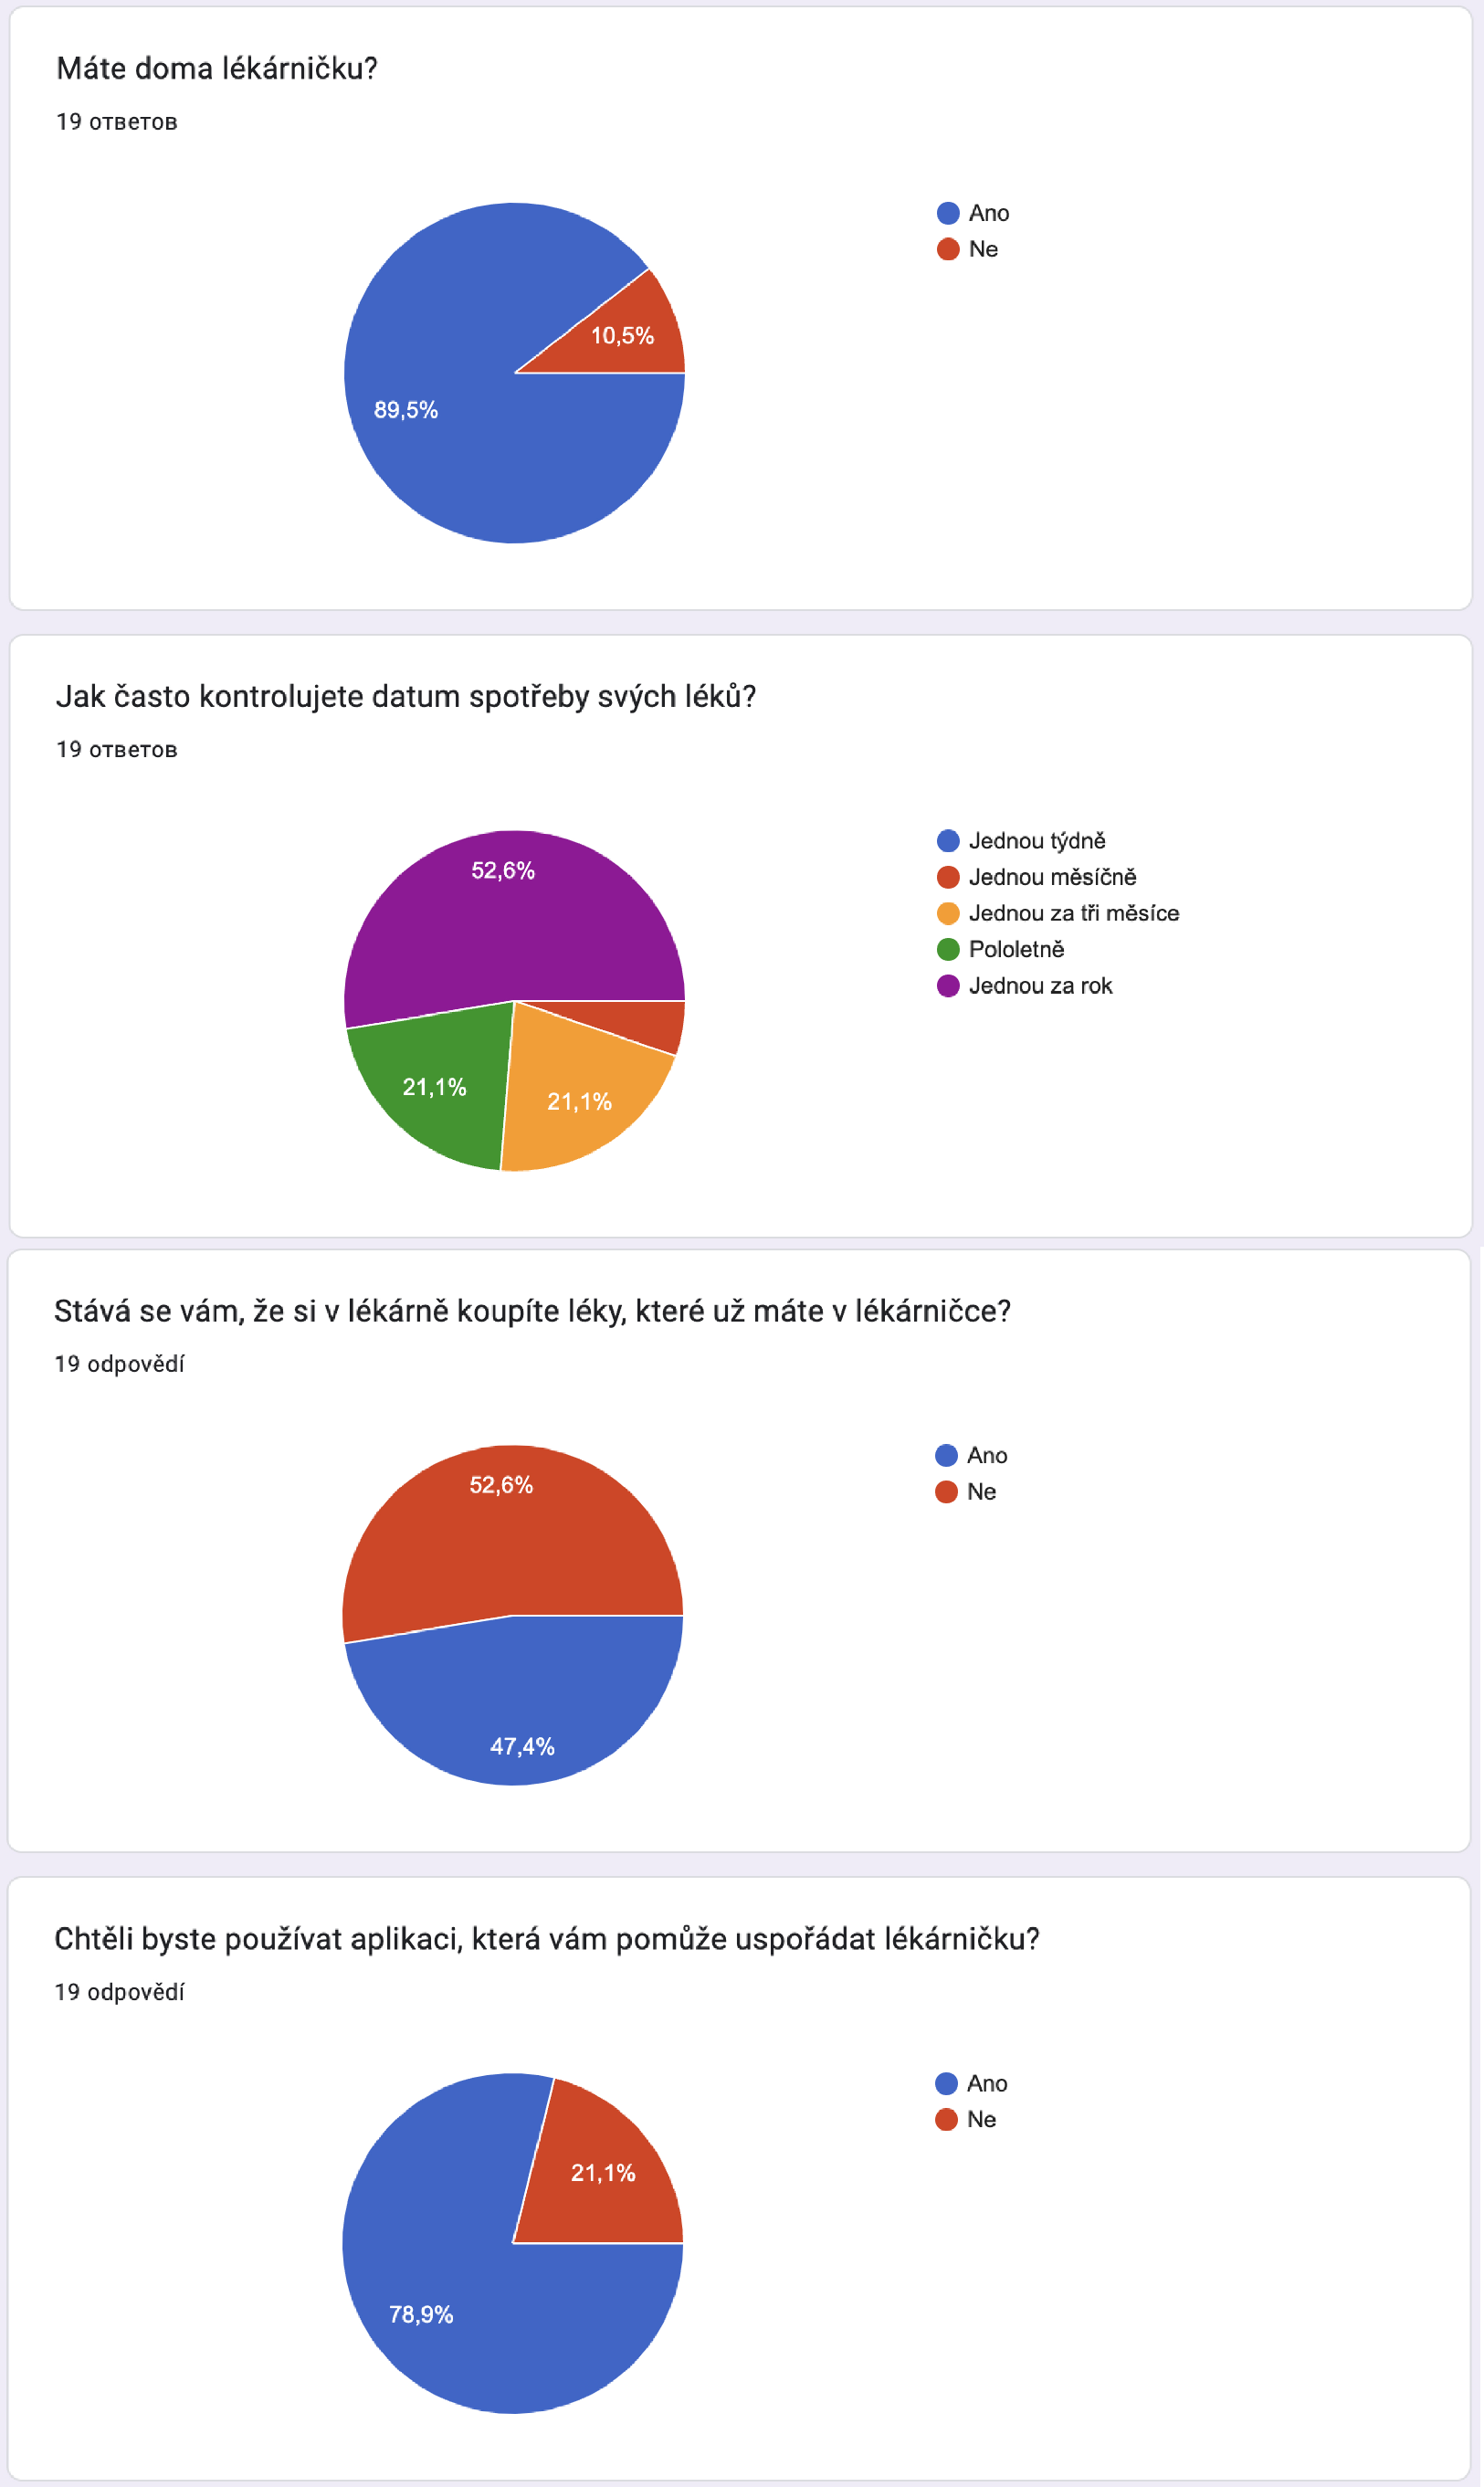
\includegraphics[width=\textwidth,height=720,keepaspectratio]{Pruzkum.pdf}
		\caption{Grafické znázornění výsledků průzkumu - 1. část}
		\label{figure:pruzkum}
	\end{figure}

 \begin{figure}[!ht]
		\centering
		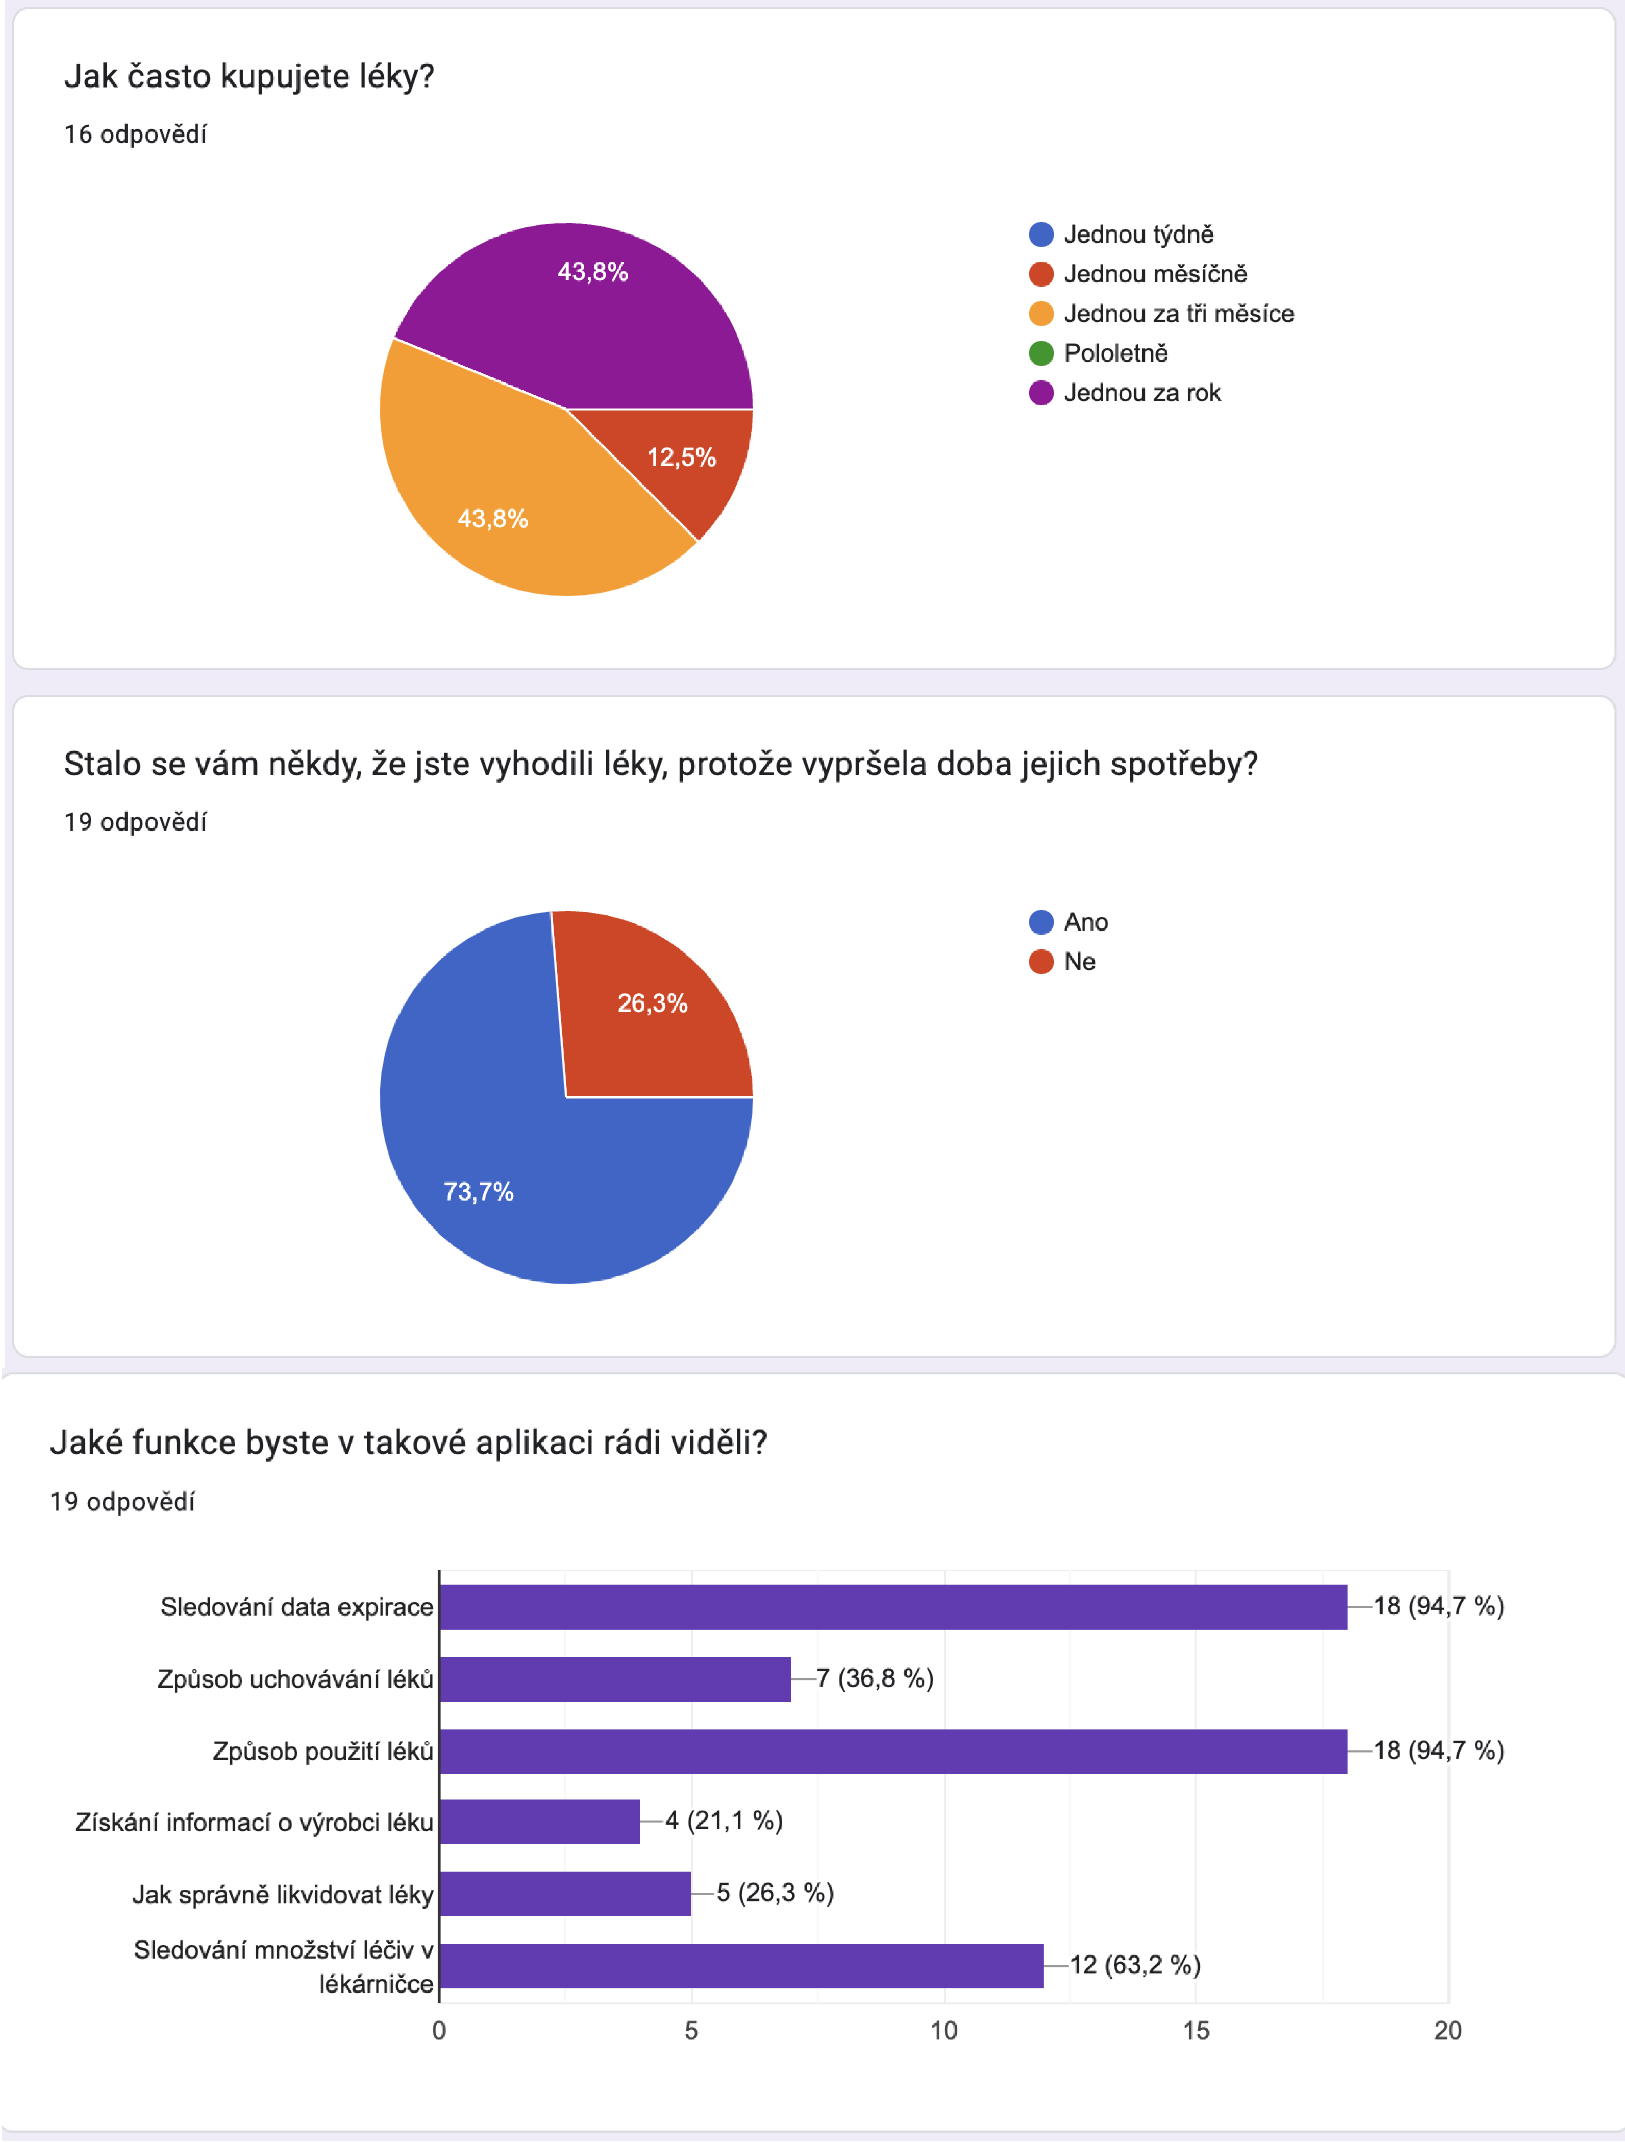
\includegraphics[width=1\linewidth]{Pruzkum1.pdf}
		\caption{Grafické znázornění výsledků průzkumu - 2. část}
		\label{figure:pruzkum1}
	\end{figure}
 \FloatBarrier

	\subsection{Existující aplikaci}
 Po provedení analýzy existujících aplikací dostupných v App Store vyšlo najevo několik společných trendů a nedostatků. Většina těchto aplikací primárně poskytuje uživatelům kalendář léků, ale postrádá komplexní sledování lékárničky. Většina těchto aplikací se navíc řídí vzorem, kdy nabízí 3denní zkušební období, po kterém se uživatelé musí přihlásit k odběru nebo provést platbu (\textbf {Figure \ref{figure:mytherapy}}).

 Jedna konkrétní aplikace, „Moje léky“, však vyniká v několika aspektech. Umožňuje uživatelům vytvářet seznamy svých léků spolu s frekvencí užívání. Navzdory tomu jsou v této aplikaci značné nedostatky. Nepodporuje sledování množství léků, neposkytuje prostředky pro přístup k návodům na užívání léků, nejsou základní upozorňovací funkce a odstává z hlediska nabídky moderního a uživatelsky přívětivého rozhraní (\textbf {Figure \ref{figure:moje leky}}).

 \begin{figure}[!ht]
		\centering	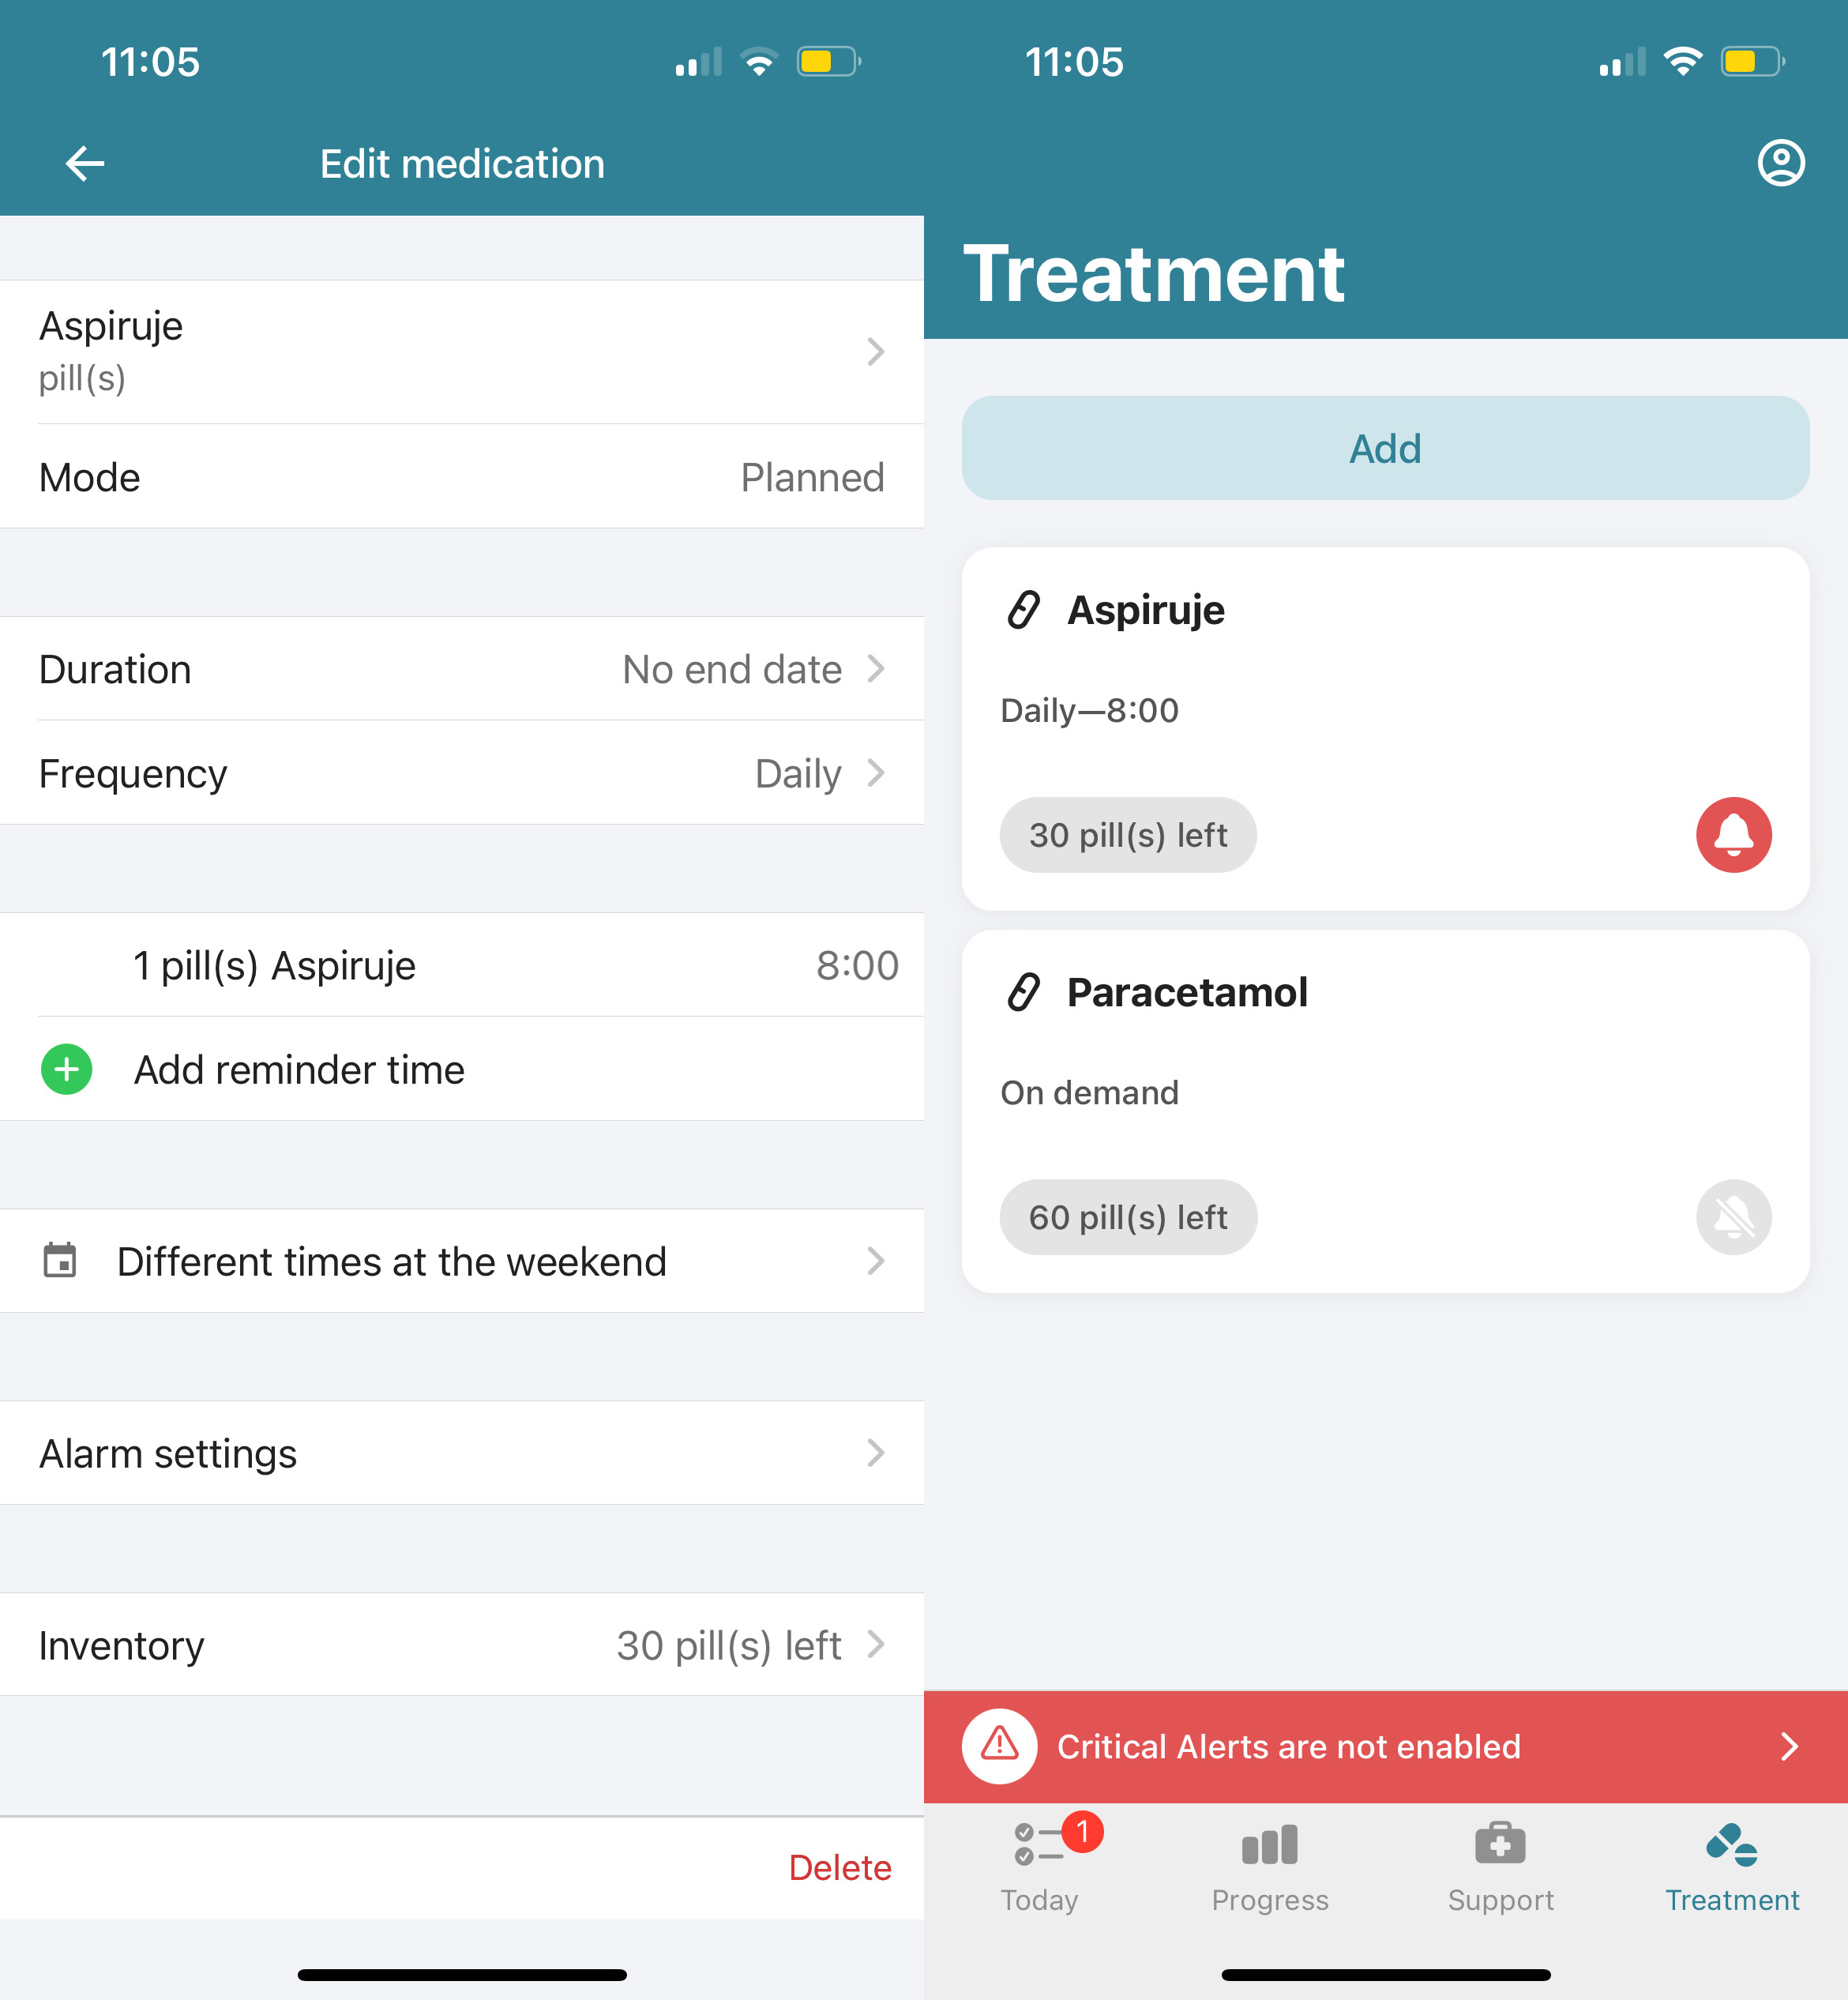
\includegraphics[width=220,height=210,keepaspectratio]{mytherapy.jpeg}
		\caption{Aplikace MyTherapy}
		\label{figure:mytherapy}
	\end{figure}
 \begin{figure}[!ht]
		\centering
		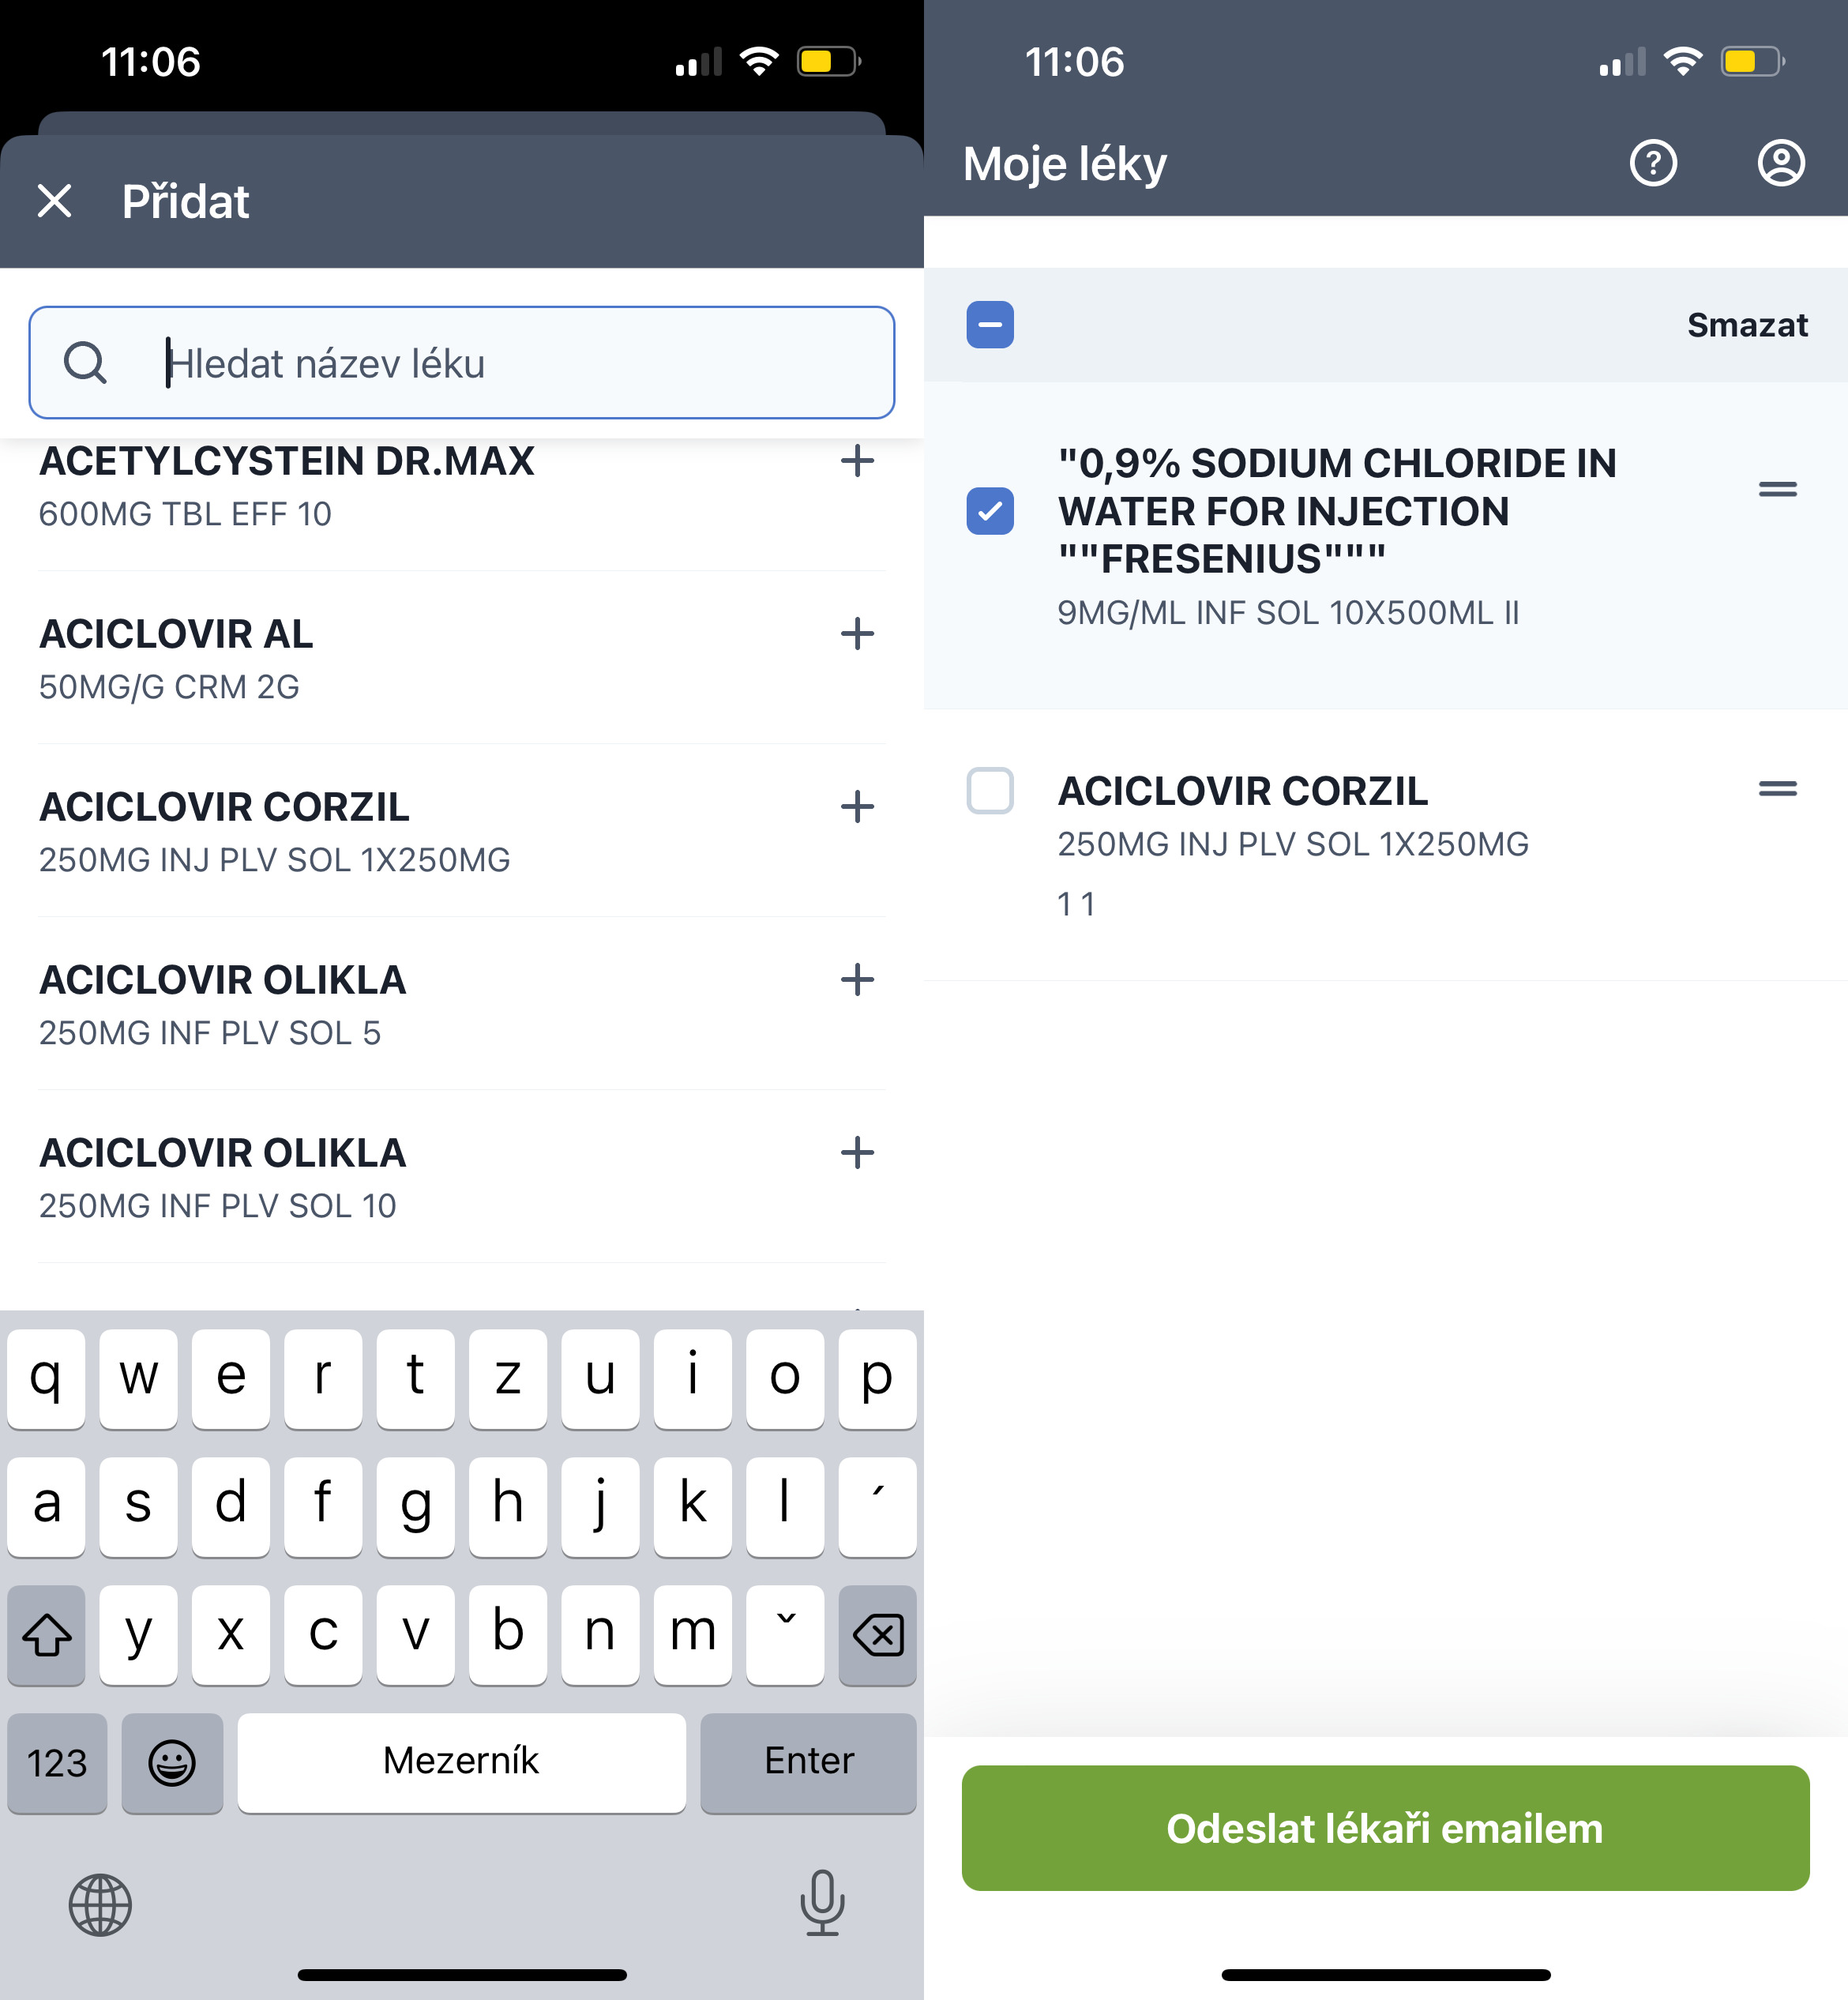
\includegraphics[width=220,height=210,keepaspectratio]{moje leky.jpeg}
		\caption{Aplikace Moje Leky}
		\label{figure:moje leky}
	\end{figure}
 \FloatBarrier

Podle těchto zjištění je evidentní příležitost vytvořit vynikající aplikaci pro sledování léků, která tato omezení řeší. Taková aplikace by se mohla odlišit tím, že poskytuje následující:
 \begin{itemize}
     \item \textbf{Komplexní sledování kabinetu léků:} Na rozdíl od konkurence by naše aplikace zahrnovala robustní systém řízení zásob léků. Uživatelé budou moci sledovat zbývající množství leků, což zajistí, že nikdy nečekaně nedojdou.
     \item \textbf{Úložiště informací o lécích:} Abychom uživatelům poskytli znalosti, naše aplikace by obsahovala rozsáhlou databázi léků. Uživatelé mohou snadno získat podrobné informace o svých lécích, jako jsou pokyny k použití, potenciální vedlejší účinky.
     \item \textbf{Rozhraní zaměřené na uživatele:} Uvědomujeme si důležitost uživatelské zkušenosti. Proto bude naše aplikace obsahovat elegantní, intuitivní a moderní rozhraní navržené tak, aby přidávání, úpravy a správa léků bylo snadné.
     \item \textbf{Chytrá upozornění a připomenutí:} Naše aplikace bude uživatelům poskytovat včasné připomenutí ohledně doplňování léků a zajistí, že budou mít přehled o zásobách léků. Tato připomenutí pomohou uživatelům efektivně spravovat své léky.
 \end{itemize}
Na závěr, naše připravovaná aplikace si klade za cíl zaplnit jasnou mezeru na trhu tím, že nabídne komplexní a uživatelsky přívětivé řešení sledování léků. Odstraněním nedostatků pozorovaných ve stávajících aplikacích a upřednostněním uživatelských potřeb se snažíme poskytovat vynikající uživatelský zážitek a nástroj, který skutečně umožňuje jednotlivcům spravovat své léky efektivně a s jistotou.



	\subsection{Analýz uživatelských potřeb}
	\textbf{Klíčové potřeby uživatelů:}
 \begin{enumerate}
     \item Sledování léků: Uživatelé potřebují způsob, jak sledovat své léky, včetně léků na předpis a volně prodejných léků.
     \item Správa data expirace: Uživatelé chtějí vědět, kdy vyprší platnost jejich léků, což jim pomáhá vyhnout se užívání neúčinných nebo potenciálně škodlivých léků.
     \item Dostupnost: Uživatelé vyžadují možnost přístupu k informacím o lécích z různých míst, například doma, v autě a na cestách.
     \item Připomenutí a upozornění: Uživatelé potřebují včasné připomenutí a upozornění na náplně a na to, kdy vyprší platnost léků.
     \item Informace o lécích: Uživatelé hledají podrobné informace o každém léku, včetně pokynů k dávkování, vedlejších účinků.
 \end{enumerate}
\textbf{Uživatelské procesy:}
\begin{enumerate}
    \item Zadání léků: Uživatelé by měli mít možnost snadno přidat své léky do aplikace a uvést podrobnosti, jako je název léku, dávkování a množství.
    \item Sledování data expirace: Uživatelé potřebují způsob, jak zadat a sledovat data expirace svých léků, což jim umožní dostávat upozornění, když se blíží datum expirace.
    \item Vyhledávání informací o lécích: Uživatelé mohou chtít vyhledat informace o svých lécích, včetně pokynů k použití a potenciálních vedlejších účinků.
    \item Sledování na základě polohy: Uživatelé mohou potřebovat zaznamenat místo, kde uchovávají své léky, například „v autě“ nebo „doma“, aby si zajistili snadný přístup.
\end{enumerate}
Řešením těchto klíčových potřeb uživatelů a poskytováním těchto funkcí může aplikace „MedShelf“ pomoci lidem efektivně sledovat jejich léky a data jejich expirace na různých místech, čímž podporuje lepší řízení zdraví a dodržování léků.

    \section{Návrh aplikace}
Rozdělení práce spočívá v tom, že každý člen týmu se specializuje na určitou část vývoje aplikace, což nakonec vede k dokončení jediné celistvé aplikace.

	\subsection{Maketa}
  \textbf {Návrhy aplikace v nástroji Figma:}

Všichni členové našeho týmu se zapojili do procesu návrhu aplikace "MedShelf" pomocí nástroje Figma. Tento nástroj umožňuje vytvářet detailní wireframy a prototypy, což nám umožnilo vizualizovat strukturu a vzhled aplikace. Každý návrh byl pečlivě promyšlen, zohledňující jak technické, tak uživatelské aspekty.


	\subsubsection{Testování makety}
\textbf{Použité metriky}
\begin{enumerate}
    \item \textbf{Čas na splnění úkolu:} Měřili jsme, jak dlouho trvá uživatelům splnit různé úkoly v aplikaci (dokončení registrace, výběr lékárničky, prohlížení léků), což nám poskytuje informaci o efektivitě a rychlosti použití.
    \item \textbf{Zpětná vazba uživatelů:} Sbírali jsme názory a komentáře od uživatelů během a po testování, abychom získali cennou zpětnou vazbu týkající se uživatelského rozhraní, funkcionality a designu.
\end{enumerate}

\textbf{Testovací úlohy/scénáře}
\begin{enumerate}
    \item \textbf{Registrovat se v aplikaci:} Uživatel byl požádán, aby se zaregistroval v aplikaci a vyplnil základní informace (implementován na základě kostry aplikace).
    \item \textbf{Vybrat lékárničku:} Uživatel byl požádán, aby vybral konkrétní lékárničku v aplikaci. To zahrnovalo navigaci a výběr lékárničky, kterou chtěl použít (implementován na základě prototypu aplikace).
    \item \textbf{Zobrazit léky z lékárničky a vyhodnotit snadnost prezentace informací:} Uživatel měl za úkol zobrazit léky, které byly uloženy v dané lékárničce, a posoudit, zda prezentace informací o léku byla snadná a srozumitelná. Tato úloha pomohla zjišťovat potenciální nedostatky v zobrazování léků.
    \item \textbf{Hledat informace o léku:} Uživatel byl vyzván, aby vyhledal informace o konkrétním léku v aplikaci. To zahrnovalo použití funkce vyhledávání a posouzení, jak dobře a rychle bylo možné najít potřebné informace.

\end{enumerate}

\textbf{Testovaní subjekti:}

Pro testování jsme zvolili 9 různorodých subjektů, zahrnujících osoby různého věku, pohlaví a úrovně technických dovedností. To nám umožnilo získat různorodý pohled na aplikaci a zajistit, že bude vhodná pro různé uživatelské skupiny.

\textbf{Průběh testování:}

Testování probíhalo pod dohledem jednoho ze členů týmu, který pozoroval, jak subjekt plní zadané úkoly. Během testování jsme sbírali data o časech na splnění úkolů a pozorovali jsme, jak uživatelé interagují s maketou aplikací. Dále jsme zaznamenávali jejich zpětnou vazbu a komentáře.

Sbíraný feedback a identifikované nedostatky nám umožnily zlepšit aplikaci a zajistit, že bude co nejlepší pro uživatele. Testování makety bylo klíčovým prvkem našeho vývojového procesu, a budeme pokračovat v zlepšování naší aplikace na základě další zpětné vazby od uživatelů.

Byla testována maketa každého člena týmu, byly uvedeny výhody a nevýhody každé makety.

   \subsubsection{Maketa Nikita Moiseev}
\noindent \textbf{Nedostatky makety aplikace:}
   \begin{itemize}
       \item Nepohodlný seznam léků: Testování ukázalo, že seznam léků v aplikaci není pohodlný pro uživatele. To může zahrnovat nejasné zobrazení, obtížnosti při přidávání nebo editaci léků, nebo špatnou organizaci seznamu léků. Tento problém může způsobit frustraci uživatelů a snížit jejich spokojenost s aplikací.
       \item Zastaralá spodní lišta: zjištěná zastaralá spodní lišta může zahrnovat prvky, které uživatelé nepovažují za užitečné nebo důležité. To může způsobit zmatek a nepřehlednost v navigaci aplikace, což je závažný nedostatek.
   \end{itemize}
   \textbf{Výhody  makety aplikace:}
   \begin{itemize}
       \item Dostupnost vyhledávání: Přítomnost vyhledávacího nástroje může uživatelům usnadnit rychlé nalezení konkrétního obsahu nebo informací v aplikaci. To zlepšuje uživatelskou zkušenost a efektivitu použití.
       \item Přítomnost záložek: Záložky umožňují uživatelům snadný přístup k různým lekárničkam. To zlepšuje organizaci obsahu a umožňuje rychlý přechod mezi různými částmi aplikace.
       \item Pohodlné přihlášení a registrace: Snadný a pohodlný proces přihlášení a registrace je klíčovým faktorem pro získání nových uživatelů a udržení stávajících. Testování ukazuje, že tento aspekt je v aplikaci úspěšný (\textbf {Figure \ref{figure:maketa1}}).
   \end{itemize}
   \begin{figure}[!ht]
		\centering	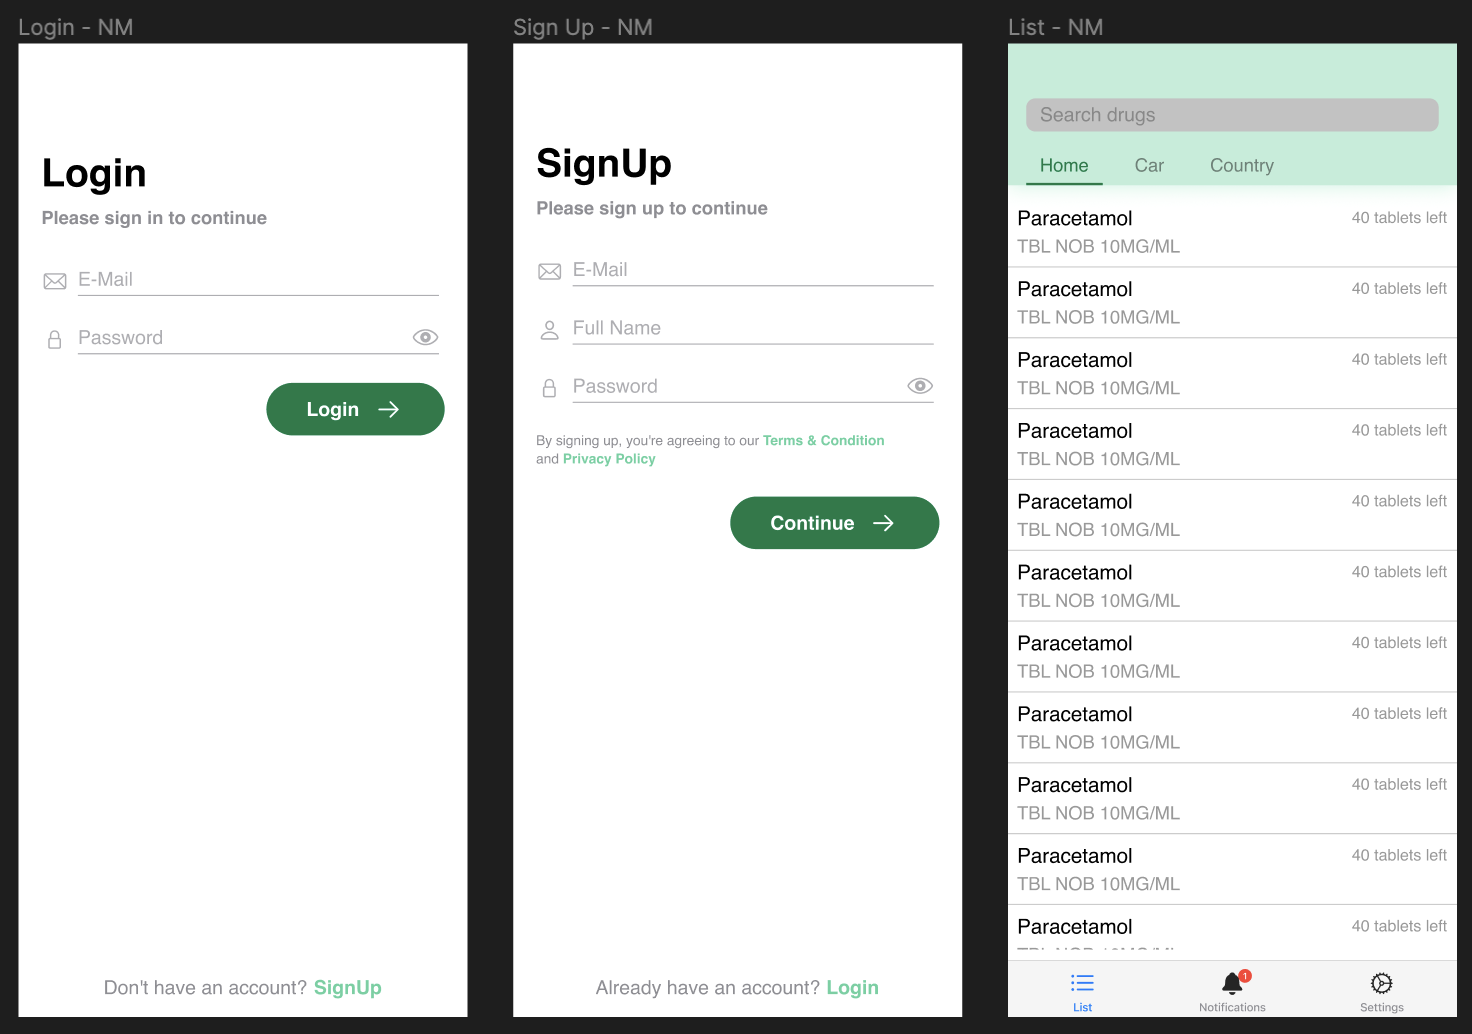
\includegraphics[width=\textwidth,height=\textheight,keepaspectratio]{Maketa_NM.png}
		\caption{Maketa 1. Autor Nikita Moiseev}
		\label{figure:maketa1}
	\end{figure}
\FloatBarrier

   \subsubsection{Maketa Nikita Pasynkov}
\noindent \textbf{Nedostatky makety aplikace:}
   \begin{itemize}
       \item Tmavé téma aplikace: Tmavé téma aplikace může způsobovat problémy nebo nepohodlí některým uživatelům, zejména těm, kteří preferují světlé pozadí. Toto rozhodnutí může ovlivnit komfort používání aplikace a čitelnost obsahu.
       \item Chybí spodní lišta, přítomno boční menu: uživatelé vnímají boční menu jako méně pohodlné než spodní lištu, může to ovlivnit uživatelskou přívětivost aplikace.
   \end{itemize}
   \textbf{Výhody  makety aplikace:}
   \begin{itemize}
       \item Dostupnost vyhledávání: Přítomnost vyhledávacího nástroje může uživatelům usnadnit rychlé nalezení konkrétního obsahu nebo informací v aplikaci. To zlepšuje uživatelskou zkušenost a efektivitu použití.
       \item Karty pro každý lék: Použití karet pro každý lék může pomoci uživatelům rychle identifikovat a navigovat mezi různými léky. Karty mohou zlepšit organizaci obsahu a usnadnit uživatelům správu svých léků (\textbf {Figure \ref{figure:maketa2}}).
   \end{itemize}
   \begin{figure}[!ht]
		\centering	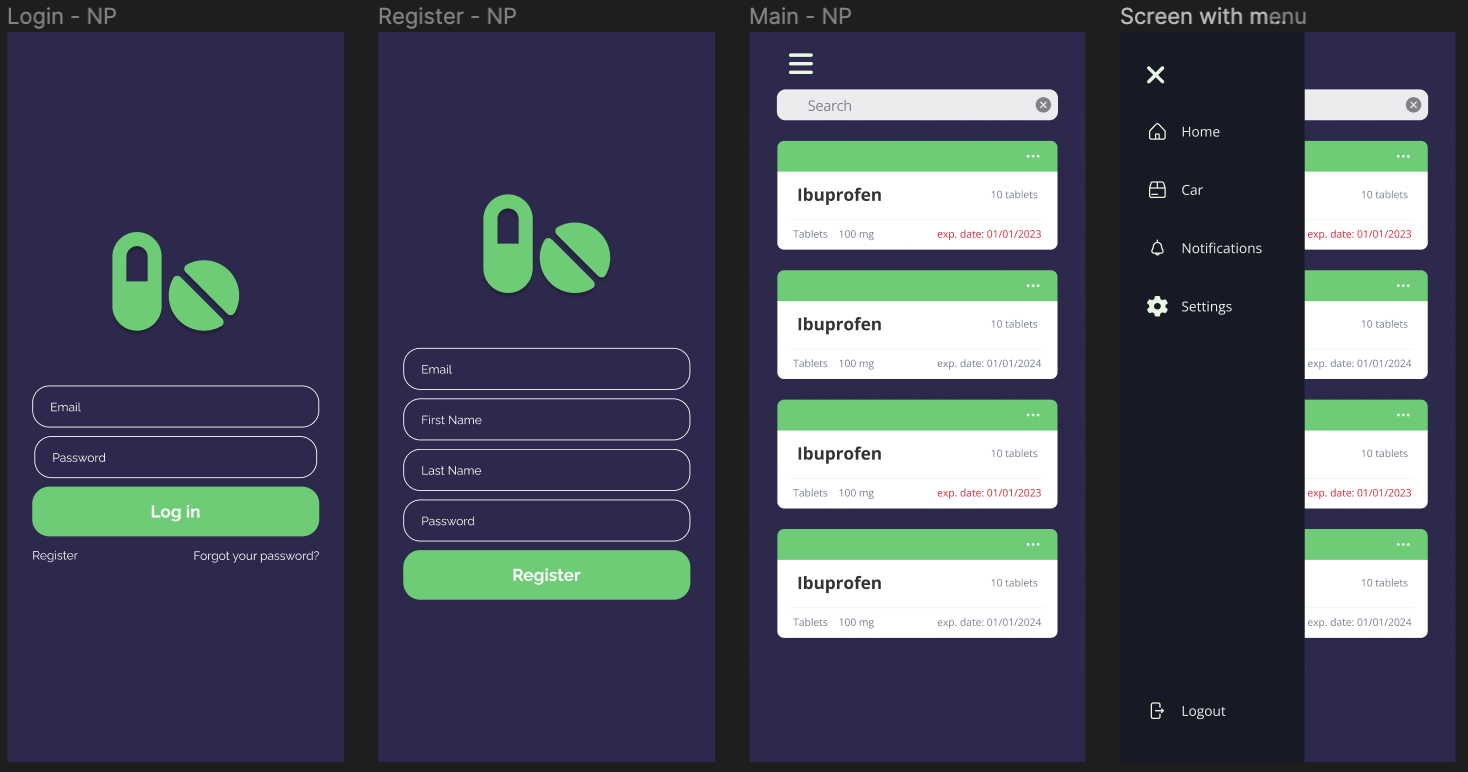
\includegraphics[width=\textwidth,height=\textheight,keepaspectratio]{Maketa_NP.png}
		\caption{Maketa 2. Autor Nikita Pasynkov}
		\label{figure:maketa2}
	\end{figure}
 \FloatBarrier

   \subsubsection{Maketa Elena Marochkina }
\noindent \textbf{Nedostatky makety aplikace:}
   \begin{itemize}
       \item Nedostatek hledání: Během testování bylo zjištěno, že aplikace trpí nedostatečným nebo neefektivním vyhledáváním. To může způsobit frustraci uživatelů, kteří hledají konkrétní léky nebo informace. Je důležité zvážit, jakým způsobem zlepšit vyhledávací funkce aplikace, aby byly snadno dostupné a efektivní pro uživatele.
       \item Nepohodlná navigace mezi lékárničkami: Testování ukázalo, že navigace mezi lékárničkami v aplikaci není pohodlná. Uživatelé mohou být zmatení nebo najít obtíže při přecházení mezi různými částmi aplikace. Toto je závažný nedostatek, který by měl tým pečlivě zvážit, protože snadná a pohodlná navigace je klíčovým faktorem pro pozitivní uživatelskou zkušenost.
   \end{itemize}
   \textbf{Výhody  makety aplikace:}
   \begin{itemize}
       \item Moderní spodní lišta: Pozitivní zpětná vazba na moderní spodní lištu ukazuje, že uživatelé jsou spokojeni s touto částí rozhraní. Moderní design a rozhraní mohou vytvořit pozitivní dojem a zvýšit atraktivitu aplikace.
       \item Nejlepší design podle uživatelů (barevný rozsah): Když uživatelé označili design aplikace za nejlepší, znamená to, že barvy a celkový vizuální dojem byly velmi příjemné. Tato pozitivní zpětná vazba by měla být zachována a zdokonalena, aby uživatelé byli spokojeni s vizuálním vzhledem aplikace (\textbf {Figure \ref{figure:maketa3}}).
   \end{itemize}
   \begin{figure}[!ht]
		\centering	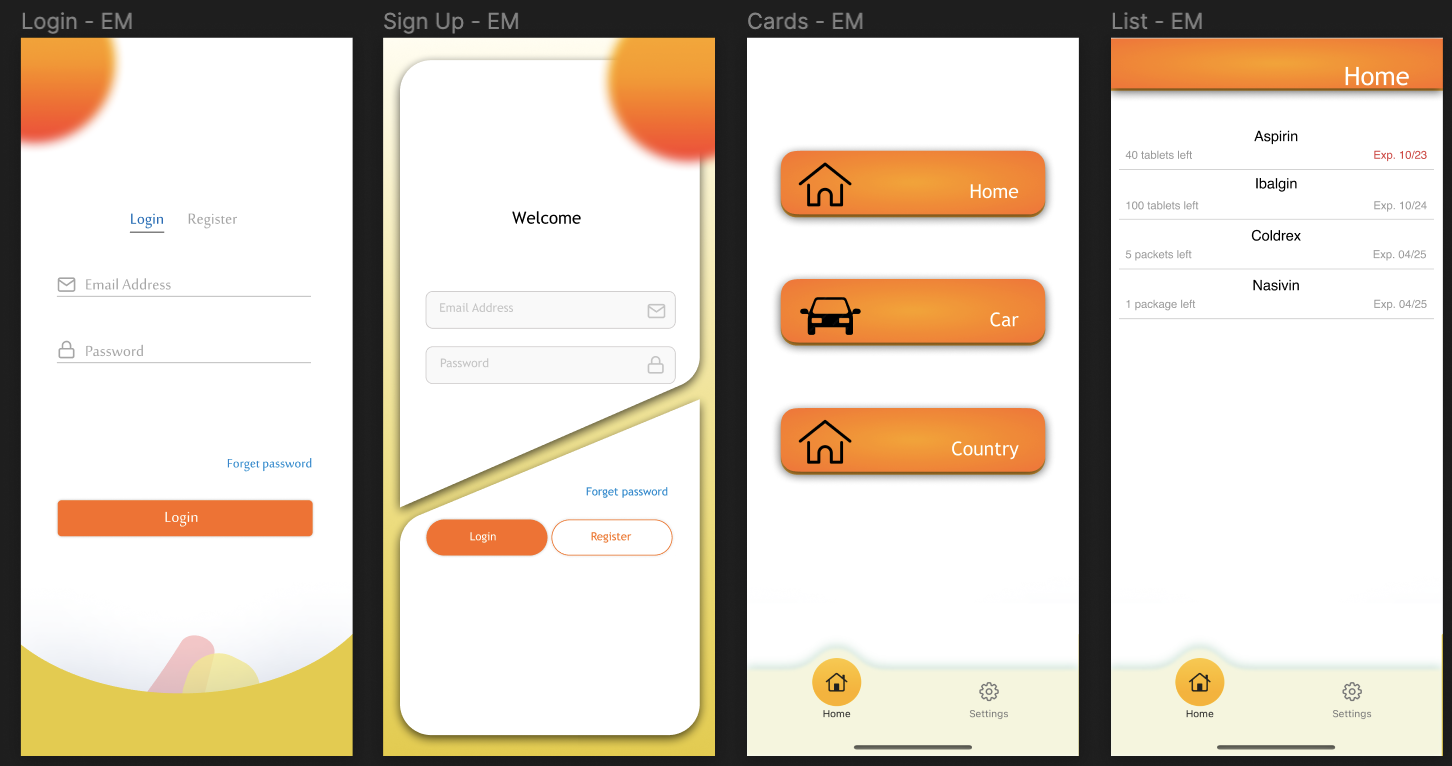
\includegraphics[width=\textwidth,height=\textheight,keepaspectratio]{Maketa_EM.png}
		\caption{Maketa 3. Autor Elena Marochkina}
		\label{figure:maketa3}
	\end{figure}

\FloatBarrier

   \subsubsection{Společná Maketa}
    Společná maketa v sobě spojuje všechny přednosti maket jednotlivých týmů a současně odstraňuje jejich nedostatky. Tato komplexní maketa byla vytvořena tak, aby poskytovala optimální kombinaci designu, funkcionalit a efektivity, zohledňující zpětnou vazbu uživatelů a potřeby projektu (\textbf {Figure \ref{figure:spolecnamaketa}}).
   \begin{figure}[!ht]
		\centering	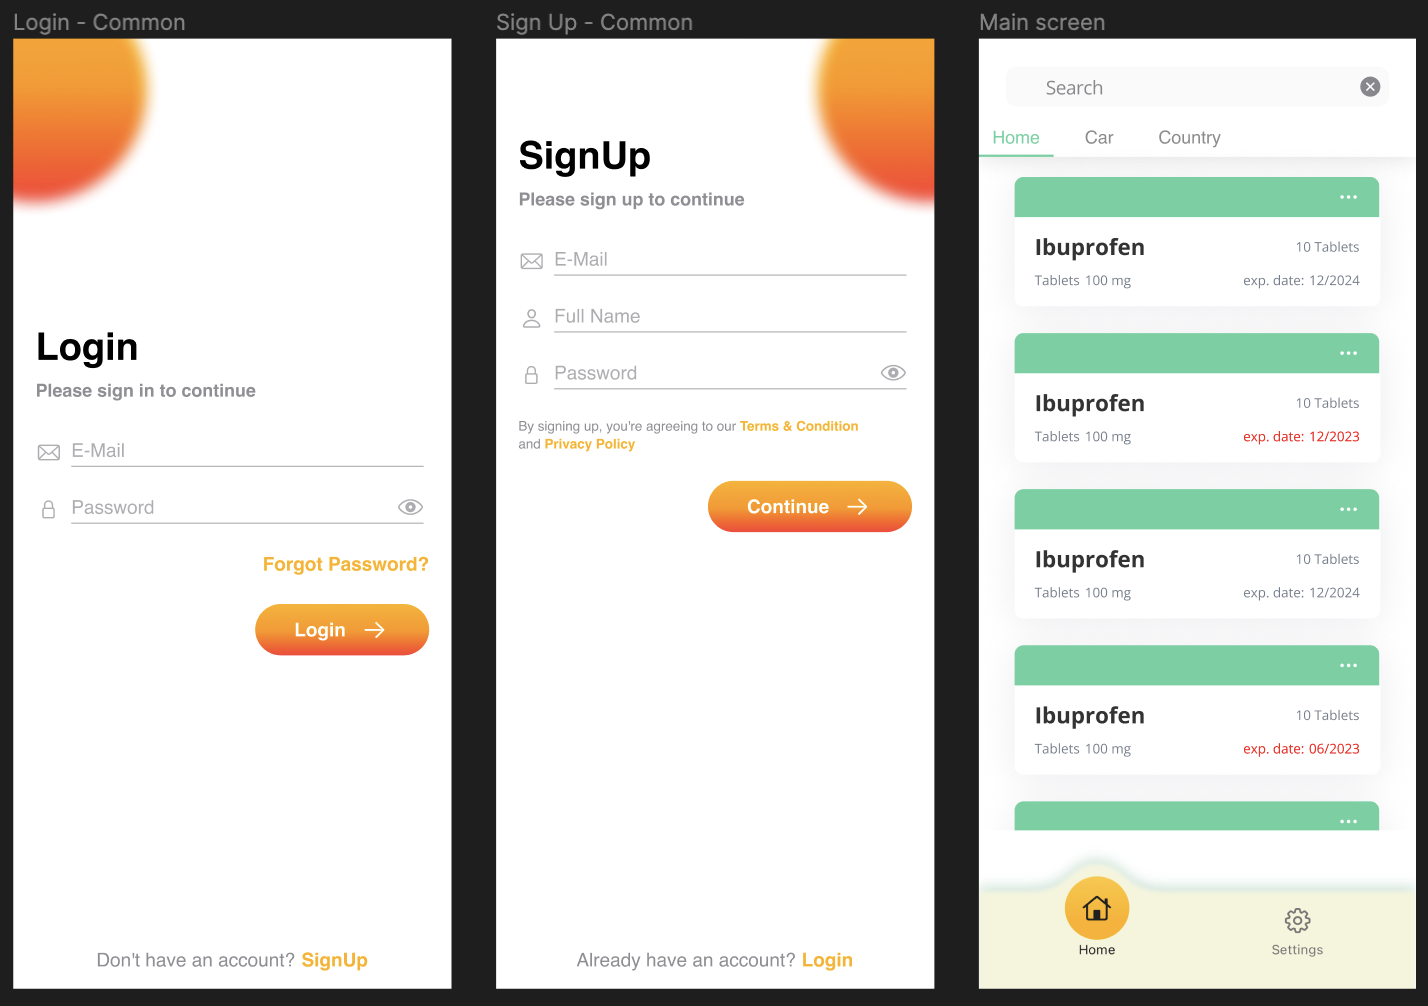
\includegraphics[width=\textwidth,height=\textheight,keepaspectratio]{Common_Maket.png}
		\caption{Společná Maketa}
		\label{figure:spolecnamaketa}
	\end{figure}

\FloatBarrier

\subsection{Architektura aplikace}
\subsubsection{Backend}
 Backend je implementován pomocí Headless CMS s názvem Directus. Tento systém má vestavěné rozhraní pro práci s vlastními entitami, uživateli, přístupovými právy a soubory.

\paragraph{Entity}
Administrační panel systému umožňuje vytvářet entity, včetně správy polí entit a propojení mezi entitami. Po vytvoření entit se automaticky vytvoří základní operace CRUD (Create/Read/Update/Delete) pro práci s nimi.

Operace je přístupná přes koncový bod

\code {items/:entity\_name/:entity\_id?}
\begin{itemize}
    \item \code {entity\_name} - název vytvořené entity, který je ekvivalentní názvu tabulky v databázi
    \item \code {entity\_id} je unikátní identifikátor entity, který je uložen v databázi ve formátu primárního klíče. Tento parametr je uveden pouze při aktualizaci nebo odstranění entity nebo získání konkrétní instance této entity.
\end{itemize}

Operace CRUD na entitě je určena metodou požadavku HTTP:
\begin{itemize}
  \item GET - získání entity/všech entit
  \item POST - vytvoření nové entity
  \item PUT - aktualizace existující entity
  \item DELETE - mazání entity
  \end{itemize}

Při použití metod pro vytváření nebo aktualizaci entit musí být také specifikováno tělo požadavku, které bude obsahovat všechna potřebná pole a také identifikátory pro pole jako O2M (One-To-Many), M2O (Many-To-One), M2M (Many-to-Many)

\paragraph {Uživatelé a přístupová práva}
Systém Directus má rozsáhlé vestavěné možnosti pro správu uživatelů prostřednictvím uživatelského rozhraní systému. Každý uživatel je identifikován pomocí svého unikátního identifikátoru. Každý uživatel má také svou vlastní roli. Systém rolí hraje klíčovou roli při autorizaci uživatelů v systému. Pro každou roli je možné nastavit specifická přístupová pravidla pro každou operaci CRUD na konkrétní entitě. Pravidla přístupu nejsou omezena pouze na přítomnost nebo nepřítomnost pravidla, ale mají také schopnost udělit přístup ke konkrétním polím entity a omezit přístup k určitým instancím entity na základě polí entity.

\subsubsection{Frontend}
Pro implementaci klientské části aplikace bylo rozhodnuto vytvořit aplikaci pro mobilní telefon, protože tento formát aplikace bude pro uživatele z hlediska designu, funkčnosti a mobility pohodlnější než počítačová aplikace nebo webová stránka.

\paragraph{SwiftUI}
Aplikace pro mobilní telefony cílí na platformy s operačním systémem iOS. Aplikace je napsána pomocí vestavěné knihovny Apple s názvem SwiftUI. Tato knihovna byla vytvořena a podporována společností Apple již dlouhou dobu a je jimi oficiálně propagována jako plnohodnotná alternativa k Objective-C. Navzdory skutečnosti, že některé komplexní funkce, které blíže interagují s funkčností operačního systému nebo jeho jádra, jsou dostupné pouze při použití Objective-C, byly jako jazyk pro vývoj aplikace vybrány Swift a knihovna SwiftUI, protože možnosti, které nabízejí jsou dostatečné k plné implementaci funkčnosti aplikace.

\paragraph{Architektura}
Zdrojový kód aplikace se řídí vzorem MVVM (Model-View-ViewController).

Každá datová entita, kterou aplikace obdrží z backendu, je uložena ve formátu dekódovatelné struktury. Použití rozšíření struktury pomocí Decodable umožňuje automaticky dekódovat data přijatá z backendu do formátu požadované struktury. Tyto struktury ve zdrojovém kódu provádějí přiřazení modelů ze vzoru MVVM.

Dalším bodem vzoru je View. Tato část vzoru, stejně jako předchozí, používá struktury ve Swift k implementaci funkcí. Rámce pro implementaci View jsou vždy rozšířeny o vestavěný rámec View SwiftUI, který umožňuje knihovně SwiftUI navrhovat uživatelské rozhraní pomocí existujících prvků uživatelského rozhraní v knihovně. Při návrhu všech aplikačních rozhraní vám tato knihovna umožňuje využívat principy modularity a vytvářet univerzální komponenty, které budou znovu použity na různých místech rozhraní.

Poslední část vzoru MVVM ViewModel je implementována pomocí tříd ve Swiftu a speciálních dekorátorů.

\end{document}